\documentclass{beamer}
\usepackage[utf8]{inputenc}

\usetheme{Madrid}
\usecolortheme{default}
\usepackage{amsmath,amssymb,amsfonts,amsthm}
\usepackage{txfonts}
\usepackage{tkz-euclide}
\usepackage{listings}
\usepackage{adjustbox}
\usepackage{array}
\usepackage{tabularx}
\usepackage{gvv}
\usepackage{lmodern}
\usepackage{circuitikz}
\usepackage{tikz}
\usepackage{graphicx}

\setbeamertemplate{page number in head/foot}[totalframenumber]

\usepackage{tcolorbox}
\tcbuselibrary{minted,breakable,xparse,skins}



\definecolor{bg}{gray}{0.95}
\DeclareTCBListing{mintedbox}{O{}m!O{}}{%
	breakable=true,
	listing engine=minted,
	listing only,
	minted language=#2,
	minted style=default,
	minted options={%
		linenos,
		gobble=0,
		breaklines=true,
		breakafter=,,
		fontsize=\small,
		numbersep=8pt,
		#1},
	boxsep=0pt,
	left skip=0pt,
	right skip=0pt,
	left=25pt,
	right=0pt,
	top=3pt,
	bottom=3pt,
	arc=5pt,
	leftrule=0pt,
	rightrule=0pt,
	bottomrule=2pt,
	toprule=2pt,
	colback=bg,
	colframe=orange!70,
	enhanced,
	overlay={%
		\begin{tcbclipinterior}
			\fill[orange!20!white] (frame.south west) rectangle ([xshift=20pt]frame.north west);
	\end{tcbclipinterior}},
	#3,
}
\lstset{
	language=C,
	basicstyle=\ttfamily\small,
	keywordstyle=\color{blue},
	stringstyle=\color{orange},
	commentstyle=\color{green!60!black},
	numbers=left,
	numberstyle=\tiny\color{gray},
	breaklines=true,
	showstringspaces=false,
}
%------------------------------------------------------------
%This block of code defines the information to appear in the
%Title page
\title %optional
{2.8.19}
\date{}
%\subtitle{A short story}

\author % (optional)
{M Chanakya Srinivas- EE25BTECH11036}




\begin{document}


\frame{\titlepage}




\begin{frame}{Problem Statement}
Suppose for some non-zero vector $\vec r$ we have:
\[
\vec r \cdot \vec a = 0,\quad
\vec r \cdot \vec b = 0,\quad
\vec r \cdot \vec c = 0
\]
Show that the scalar triple product $(\vec a\ \vec b\ \vec c) = 0$.
\end{frame}

\begin{frame}{Step 1: Write as Matrix Equation}
The three scalar equations can be written as:
\begin{align}
\vec r^\top \vec a &= 0 \\
\vec r^\top \vec b &= 0 \\
\vec r^\top \vec c &= 0
\end{align}

Stacked together:
\begin{align}
\myvec{
\vec a^\top \\[1mm]
\vec b^\top \\[1mm]
\vec c^\top
} \vec r = \myvec{0\\0\\0}
\end{align}
\end{frame}

\begin{frame}{Step 2: Define the Matrix}
Define the \(3\times 3\) matrix with columns $\vec a,\vec b,\vec c$:
\begin{align}
A = \big[\vec a\ \vec b\ \vec c\big]
\end{align}

Then the stacked matrix equation becomes:
\begin{align}
A^\top \vec r = \myvec{0\\0\\0}
\end{align}
\end{frame}

\begin{frame}{Step 3: Deduce Singularity}
Since $\vec r \neq \vec 0$ and 
\[
A^\top \vec r = \myvec{0\\0\\0},
\] 
the matrix $A^\top$ is singular. Therefore:
\begin{align}
\det(A^\top) = 0
\end{align}
\end{frame}

\begin{frame}{Step 4: Relate to Scalar Triple Product}
But $\det(A^\top) = \det(A)$, and the determinant of $A$ is the scalar triple product:
\begin{align}
(\vec a\ \vec b\ \vec c) = \det\big[\vec a\ \vec b\ \vec c\big] = \det(A) = 0
\end{align}
\end{frame}

\begin{frame}{Conclusion}
\[
\boxed{(\vec a\ \vec b\ \vec c) = 0}
\]

This completes the proof  **non-zero $\vec r$ orthogonal to all three vectors**.
\end{frame}





\begin{frame}[fragile]{C Code}
\begin{lstlisting}[language=C]
#include <stdio.h>

double scalar_triple(double a[3], double b[3], double c[3]) {
    return a[0]*(b[1]*c[2] - b[2]*c[1])
         - a[1]*(b[0]*c[2] - b[2]*c[0])
         + a[2]*(b[0]*c[1] - b[1]*c[0]);
}
    \end{lstlisting}
\end{frame}

\begin{frame}[fragile]{Python code through shared output}
\begin{lstlisting}
import ctypes
import matplotlib.pyplot as plt
import numpy as np
from mpl_toolkits.mplot3d import Axes3D
# Load the shared library
lib = ctypes.CDLL("./libstp.so")
lib.scalar_triple.restype = ctypes.c_double
# Define vectors
a = (ctypes.c_double * 3)(1, 0, 0)
b = (ctypes.c_double * 3)(0, 1, 0)
c = (ctypes.c_double * 3)(1, 1, 0)
# Call the C function
result = lib.scalar_triple(a, b, c)
print("Scalar triple product =", result)
# Convert to numpy arrays for plotting
a_vec = np.array([a[0], a[1], a[2]])
b_vec = np.array([b[0], b[1], b[2]])
c_vec = np.array([c[0], c[1], c[2]])
    \end{lstlisting}
\end{frame}
\begin{frame}[fragile]{Python code through shared output}
\begin{lstlisting}
# Plot vectors in 3D
fig = plt.figure()
ax = fig.add_subplot(111, projection='3d')
origin = np.array([0, 0, 0])
ax.quiver(*origin, *a_vec, color='r', label='a')
ax.quiver(*origin, *b_vec, color='g', label='b')
ax.quiver(*origin, *c_vec, color='b', label='c')
ax.set_xlim([0, 1.5])
ax.set_ylim([0, 1.5])
ax.set_zlim([0, 1.5])
ax.set_xlabel("X")
ax.set_ylabel("Y")
ax.set_zlabel("Z")
ax.set_title(f"Scalar Triple Product = {result}")
ax.legend()
plt.show()
   \end{lstlisting}
\end{frame}
\begin{frame}[fragile]{Only Python code}
\begin{lstlisting}
import numpy as np
import matplotlib.pyplot as plt
from mpl_toolkits.mplot3d import Axes3D
# Define 3 coplanar vectors (lying in xy-plane)
a = np.array([1, 1, 0])
b = np.array([1, 0, 0])
c = np.array([0, 1, 0])
# Cross product b x c
b_cross_c = np.cross(b, c)
# Scalar triple product a . (b x c)
scalar_triple = np.dot(a, b_cross_c)
# Print the scalar triple product (should be 0)
print(f"Scalar triple product: {scalar_triple:.2f}")
# Plotting
fig = plt.figure()
ax = fig.add_subplot(111, projection='3d')
 \end{lstlisting}
\end{frame}
\begin{frame}[fragile]{Only Python code}
\begin{lstlisting}
# Plot origin
origin = np.array([0, 0, 0])
# Plot vectors
ax.quiver(*origin, *a, color='r', label='Vector a', linewidth=2)
ax.quiver(*origin, *b, color='g', label='Vector b', linewidth=2)
ax.quiver(*origin, *c, color='b', label='Vector c', linewidth=2)
# Plot b x c
ax.quiver(*origin, *b_cross_c, color='orange', linestyle='dashed', label='b x c', linewidth=2)
ax.set_xlim([0, 1.5])
ax.set_ylim([0, 1.5])
ax.set_zlim([0, 1.5])
ax.set_xlabel('X')
ax.set_ylabel('Y')
ax.set_zlabel('Z')
ax.set_title(f'Scalar Triple Product = {scalar_triple:.2f}')
ax.legend()
ax.grid(True)
plt.show()
  \end{lstlisting}
\end{frame}
\begin{frame}[fragile]{PLOTS}
\begin{figure}
    \centering
    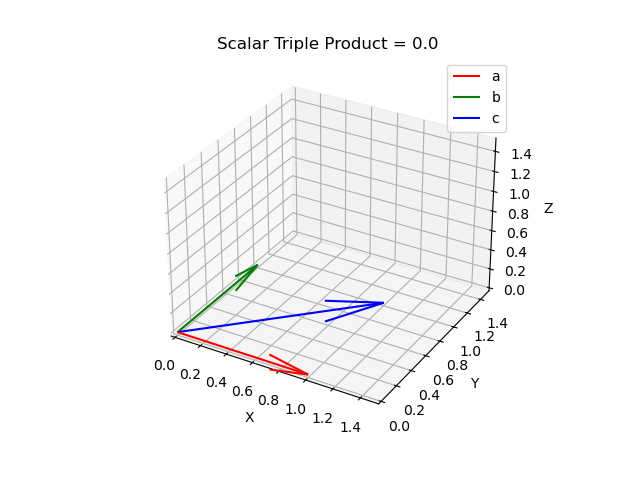
\includegraphics[width=0.9\columnwidth]{figs/fig41.png}
    \caption{}
    \label{fig:placeholder}
\end{figure}
\end{frame}
\begin{frame}[fragile]{PLOTS}
\begin{figure}
    \centering
    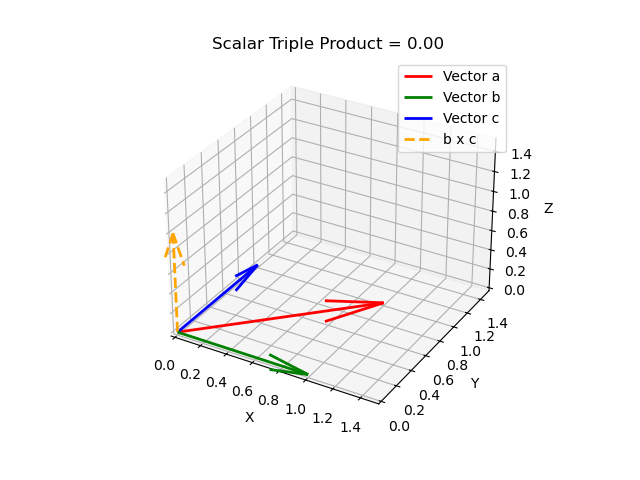
\includegraphics[width=0.9\columnwidth]{figs/fig42.png}
    \caption{}
    \label{fig:placeholder}
\end{figure}
\end{frame}
\end{document}
